\chapter{Continuity}
Assume general metric spaces $X,Y$ and $f: X\to Y$.
\begin{definition}[Definition 4.1]
	\label{def:4.1}
	Suppose $X,Y$ are metric spaces, $E \subset X$, $f: E\to Y$, $p \in E'$, where $E'$: set of limit points in metric space $X$.
	We say $\lim_{x\to p}{f(x)}=q$, or $f(x)\to q$ as $x\to p$, if $\forall_{\epsilon > 0}: \exists_{\delta>0} \text{ s.t. } (0<d_X(x,p)<\delta \text{ and } x \in E) \implies d_Y(f(x),q)<\epsilon $.
	\begin{note}
		We don't say anything about $x=p$, $f(p)$ may not even be defined.
	\end{note}
\end{definition}

% \begin{example}
% Note that we require $x$ to be in $E$.
% For instance, let the next figure represent $E \subset X$.
% \end{example}

\begin{theorem}[Theorem 4.2]
	\label{thm:4.2}
	$\lim_{x\to p}{f(x)}=q \Leftrightarrow \forall_{\{ {p}_{n}\} \text{ in } E}: \lim_{n\to \infty}{f(p_{n})}=q$ such that $p_{n}=p$ and $p_{n}\to p$, where the RHS is the limit of Definition 3.1.
	\begin{note}
		This implies uniqueness of $q$ in Definition 4.1.
	\end{note}
	\begin{proof}
		\begin{description}
			\item[$\implies $]
			      Suppose $\lim_{x\to p}{f(x)}=q$. Let $\epsilon>0$. Choose $\delta>0$ s.t. $d_Y(f(x),q)\epsilon$ if $0<d_X(x,p)<\delta$.
			      Let $\{ p_{n} \}$ be a sequence in $E$ such that $p_{n}\to p$ and $p_{n}\neq p$. Then $\exists_{N} \text{ s.t. } 0<d_X(p_{n},p)<\delta $ if $n\ge N$; i.e., $f(p_n)\to q$.
			\item[$\impliedby$]
			      Consider the contrapositive of $(\impliedby) $: $\neg(\lim_{x\to p}{f(x)}=q) \implies \neg(\forall_{\{ p_{n} \} \text{ in } E}: \lim_{n\to \infty}{f(p_{n})}=q)$.
			      Suppose $\neg(\lim_{x\to p}{f(x)}=q)$. Then $\exists_{\epsilon>0} \text{ s.t. } \forall_{\delta>0}: \exists_{x\in N_{\delta}^{E}(p)} \text{ s.t. } x\neq p \text{ and } d_Y(f(x),q)\ge \epsilon$.
			      Take $\delta=\delta_n=\frac{1}{n}$ and let $p_{n}$ be an $x$ as above for $\delta_n$. Then $p_{n}\to p$, but $d_Y(f(p_{n}),q)\ge \epsilon \forall n$, so $f(p_{n})\not \to q$.
		\end{description}
	\end{proof}
\end{theorem}

\begin{theorem}[Theorem 4.4]
	\label{thm:4.4}
	When $Y=\C$, limit as defined in Definition~\ref{def:4.1} respects sums, products and quotients.
	\begin{proof}
		By Theorem~\ref{thm:4.2}, it suffices to show that the theorem holds for sequences.
	\end{proof}
\end{theorem}

\begin{definition}
	\label{def:4.5}
	Suppose $X,Y$ are metric spaces, $p \in E \subset X$, $f: E\to Y$. Then $f$ is continuous at $p$ if $\forall_{\epsilon > 0}: \exists_{\delta > 0} \text{ s.t. } d_X(x,p)<\delta \implies d_Y(f(x),f(p))<\epsilon$; i.e., $f(N_{\delta}^{E}(p)) \subset N_{\epsilon}^{y}(f(p))$. We say $f$ is continuous if $f$ is continuous at $p$ for all $p \in E$.
	\begin{note}
		If $p$ is an isolated point; i.e., $\exists_{\delta >0} \text{ s.t. } N_{\delta}^{E}(p)=\{p\}$, then every $f: E\to Y$ is continuous at $p$.
	\end{note}
\end{definition}

\begin{theorem}[Theorem 4.6]
	\label{thm:4.6}
	Suppose $E \subset X, p \in E \cap E', f: E\to Y$. Then $f$ is continuous at $p$ if and only if $\lim_{x\to p}{f(x)}=f(p)$.
	\begin{proof}
		By Definition~\ref{def:4.1} and Definition~\ref{def:4.5} with $q=f(p)$.
	\end{proof}
\end{theorem}

\begin{theorem}[Theorem 4.7]
	\label{thm:4.7}
	For $E \subset  X, f: E\to Y, g: f(E)\to Z$, let $h=g \circ f: E\to Z$. If $f$ is continuous at $p \in E$ and if $g$ is continuous at $f(p) \in Y$, then $h$ is continuous at $p$.
	\begin{proof}
		Choose $\eta>0$ such that $d_{Y}(f(p),y)<\eta \implies d_{Z}(g(f(p)),g(y))<\epsilon$ (continuity of $g$ at $f(p)$).
		Choose $\delta>0$ s.t. $d_E(x,p)<\delta \implies d_Y(f(x),f(p))<\eta$ (continuity of $f$ at $p$).
		Then $d_E(x,p)<\delta \implies d_Z(g(f(x)),g(f(p)))=d_Z(h(x),h(p))<\epsilon$.
	\end{proof}
	% \begin{note}
	% Proof is essentially the following diagram:
	% \begin{center}
	% \begin{tikzcd}
	% 	E \arrow[r, "f"] \arrow[rd, "h=g\circ f"'] & f(E) \arrow[d, "g"] \\
	% 	& Z
	% \end{tikzcd}
	% \end{center}
	% \end{note}
\end{theorem}

\begin{theorem}[Theorem 4.8: Topological Characterization of Continutiy]
	\label{thm:4.8}
	$f: X\to Y$ is continuous $\Leftrightarrow  f^{-1}(V)$ is open for every open $V \subset Y$.
	\begin{proof}
		\begin{description}
			\item[$(\implies)$]
			      Suppose $f$ is continuous. Let $V \subset Y$ be open. Then $f^{-1}(V)$ is open.
			      Let $p \in f^{-1}(V)$. We need to show {$\exists_{\delta >0} \text{ s.t. } \linebreak N_{\delta}^{X}(p) \subset f^{-1}(V)$.} Since $V$ is open, $\exists_{\epsilon > 0} \text{ s.t. } N_{\epsilon}^{Y}(f(p)) \subset V$.
			      Since $f$ is continuous, $\exists_{\delta > 0} \text{ s.t. } f(N_{\delta}^{X}(p)) \subset N_{\epsilon}^{Y}(f(p)) \subset V$.
			      % 	  Then $f(p) \in V$. Since $V$ is open, $\exists_{\epsilon>0} \text{ s.t. } N_{\epsilon}^{Y}(f(p)) \subset V$.
			      %       Since $f$ is continuous at $p$, $\exists_{\delta>0} \text{ s.t. } f(N_{\delta}^{X}(p)) \subset N_{\epsilon}^{Y}(f(p)) \subset V$.
			      %       Thus, $N_{\delta}^{X}(p) \subset f^{-1}(V)$, so $f^{-1}(V)$ is open.
			\item[$(\impliedby)$]
			      Suppose $f^{-1}(V)$ is open for every open $V \subset Y$. Let $p \in X$ and $\epsilon>0$. Then $N_{\epsilon}^{Y}(f(p))$ is open, so $f^{-1}(N_{\epsilon}^{Y}(f(p)))$ is open. Take $V=N_{\epsilon}^{Y}(f(p))$, which is open.
			      Since $f^{-1}(V)$ is open and $p \in f^{-1}(V)$, there exists $\delta>0$ such that $N_{\delta}^{X}(p) \subset f^{-1}(V)$. Then $f(N_{\delta}^{X}(p)) \subset V=N_{\epsilon}^{Y}(f(p))$; i.e., $f$ is continuous at $p$.
		\end{description}
	\end{proof}
	\begin{remark}\hfill
		\begin{enumerate}
			\item
			      \hfill\\
			      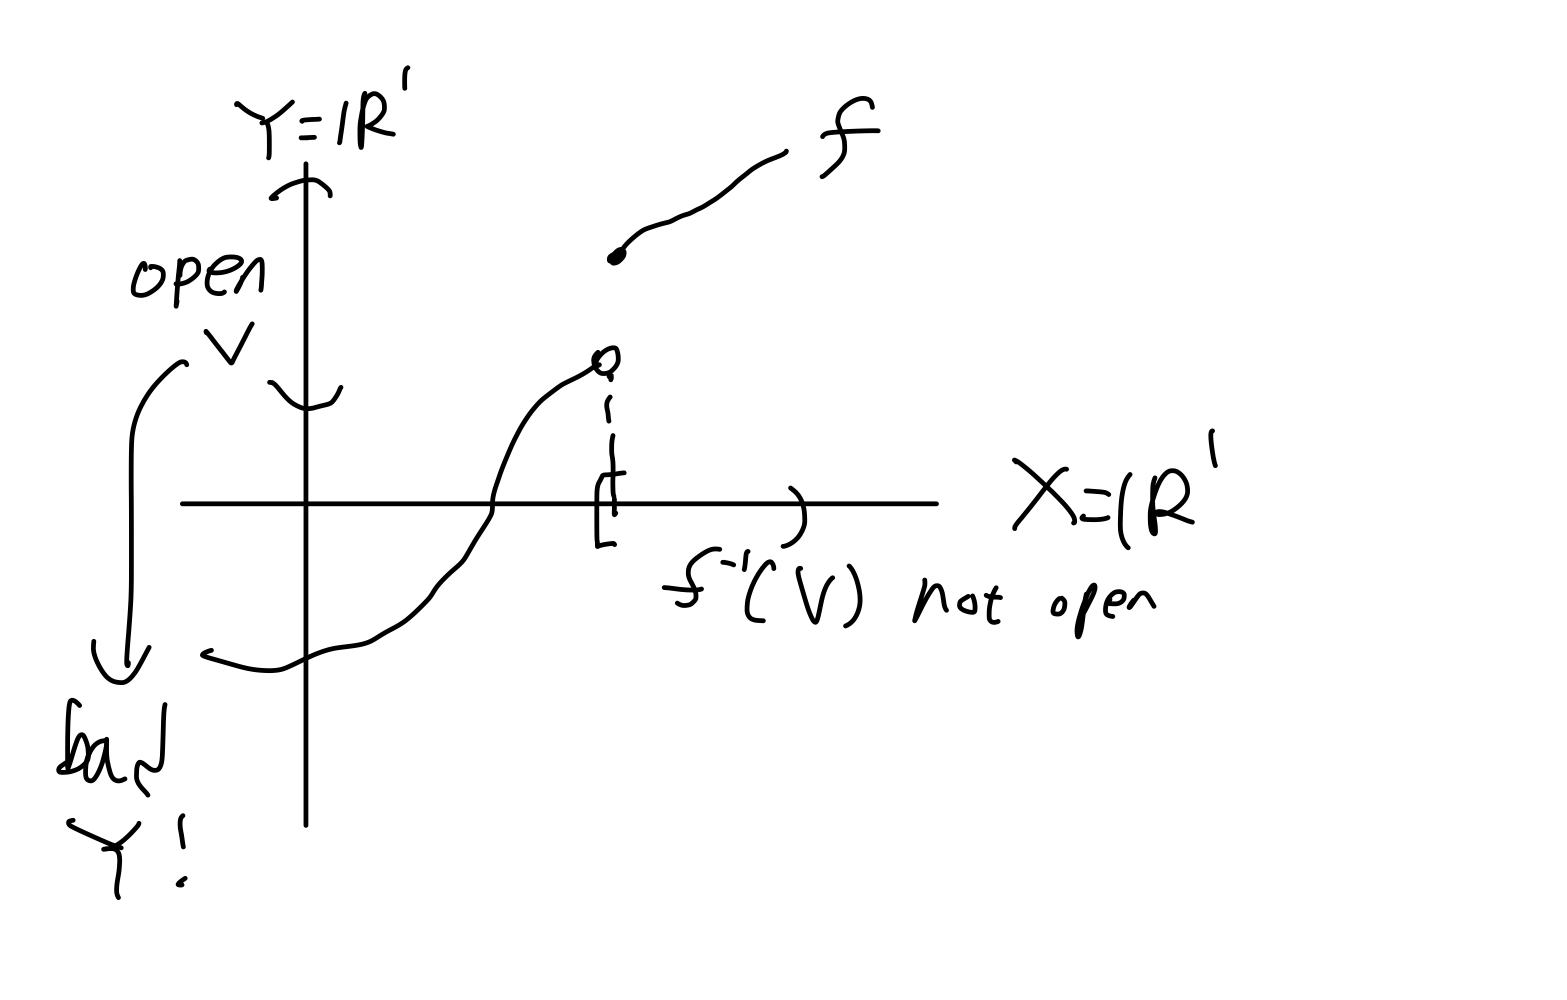
\includegraphics[width=0.5\textwidth]{./figs/thm4-8-a.jpeg}
			\item Continuity is determined by the open sets, not the metric. For instance, if metrics $l_1,l_2,l_{\infty}$ have the same open sets in $\R^{k}$, hence the same continuous functions.
			      \[
				      l_1(x,y)=\sum_{i=1}^{k}{|x_i-y_i|}
			      \]
			      \[
				      l_2(x,y)=\sqrt{\sum_{i=1}^{k}{(x_i-y_i)^2}}
			      \]
			      \[
				      l_{\infty}(x,y)=\max_{1\le i\le k}{|x_i-y_i|}
			      \]
			\item $f$ with open $U \subset X \implies f(U)$ is open are called open maps. Continuous maps need not be open(e.g., $f(x)=\text{some constant}$, $f(x)=x^2$), and open maps need not be continuous(e.g., floor function: $\left\lfloor \cdot \right\rfloor: \R\to \Z$).
		\end{enumerate}
	\end{remark}
\end{theorem}

\begin{corollary}
	$f:X\to Y$ is continuous if and only if $f^{-1}(F)$ is closed for every closed $F \subset Y$.
	\begin{proof}
		Let $V \subset Y$ be open and $F=V^{c}$. Then the above condition (RHS) is the same as $f^{-1}(V)=f^{-1}(F^{c})=(f^{-1}(F))^{c}$ is open.
	\end{proof}
\end{corollary}
